\chapter{Rancangan, Implementasi, dan Pengujian}

\section{Perancangan Perangkat Lunak} \label{PerancanganPL}
Subbab perancangan perangkat lunak menjelaskan deskripsi aplikasi, analisis kebutuhan fungsional dan non-fungsional, desain perangkat lunak, serta interaksinya.

	\subsection{Deskripsi Umum Kakas}
	Kakas pengumpulan data yang dibuat merupakan pengembangan terhadap aplikasi \textit{spreadsheet} kolaboratif yang sudah ada sebelumnya yakni EtherCalc. Kakas yang ditambahkan ini yang akan melakukan pengaturan koneksi ke basis data. Saat pengguna menginginkan penyimpanan data ke dalam basis data yang dituju, kakas ini akan melakukan pencarian bagian label dan data dan melakukan validasi masukan sebelum memasukkan data ke dalam basis data. 

	\subsection{Spesifikasi Kebutuhan}
	Pada subbab ini akan dipaparkan \textit{use case} kakas yang akan dibuat serta kebutuhan fungsional dan non-fungsional dari kakas. Kasus penggunaan oleh pengguna diberi ID dengan format UC-XX dengan UC menyatakan \textit{use case} dan XX menyatakan nomor. Pengguna adalah pihak yang menggunakan aplikasi \textit{spreadsheet} yang sudah ditambahkan kakas pengumpulan data. Kasus penggunaan oleh pengguna dijelaskan pada Tabel \ref{KebutuhanPengguna}.

	\begin{small}
	\begin{longtable}{ | p{2cm} | p{10cm} | }
	    \caption{Kasus Penggunaan oleh Pengguna}
	    \label{KebutuhanPengguna}\\ \hline
	    \centering\bfseries{ID} & \centering\bfseries{Deskripsi} \tabularnewline \hline
	    \endfirsthead
	    \hline
	    \centering\bfseries{ID} & \centering\bfseries{Deskripsi} \tabularnewline \hline
	    \endhead
	    UC-01 & Pengguna dapat menentukan basis data tujuan dengan konfigurasi basis data yang diinginkan. \\ \hline
	    UC-02 & Pengguna dapat menyimpan data yang dikumpulkan ke dalam basis data pada saat dibutuhkan. \\ \hline
	    UC-03 & Pengguna dapat mendefinisikan \textit{metadata table} yang ingin disimpan secara manual maupun otomatis oleh kakas. \\ \hline
	    UC-04 & Pengguna dapat mengubah metadata pada \textit{metadata table} yang ingin disimpan. \\ \hline
	    UC-05 & Pengguna dapat mendefinisikan aturan validasi data. \\ \hline
	    UC-06 & Pengguna dapat mengunggah berkas \textit{spreadsheet} ke dalam aplikasi. \\ \hline
	\end{longtable}
	\end{small}

	Untuk \textit{use case} dengan kode UC-06, sudah ditangani oleh aplikasi \textit{EtherCalc} sehingga tidak akan ditangani oleh kakas yang akan dikembangkan. Berdasarkan kasus penggunaan di atas, dirancang kebutuhan fungsional perangkat lunak yang diberi ID dengan format FR-XX dengan FR merupakan singkatan dari \textit{functional requirement} dan XX menyatakan nomor kebutuhan. Kebutuhan fungsional dijelaskan pada Tabel \ref{KebutuhanFungsional}.

	\begin{small}
	\begin{longtable}{ | p{2cm} | p{6cm} | p{4cm} | }
	    \caption{Kebutuhan Fungsional Kakas}
	    \label{KebutuhanFungsional}\\ \hline
	    \centering\bfseries{ID} & \centering\bfseries{Deskripsi} & \centering\bfseries{ID Use Case Terkait} \tabularnewline \hline
	    \endfirsthead
	    \hline
	    \centering\bfseries{ID} & \centering\bfseries{Deskripsi} & \centering\bfseries{ID Use Case Terkait} \tabularnewline \hline
	    \endhead
	    FR-01 & Kakas dapat melakukan koneksi kepada basis data yang ditentukan oleh pengguna melalui data masukan berupa \textit{host}, \textit{port}, \textit{username}, \textit{password}, dan \textit{database} dari basis data yang dituju. & UC-01 \\ \hline
	    FR-02 & Kakas dapat melakukan perintah basis data kepada basis data yang dituju. & UC-01, UC-02 \\ \hline
	    FR-03 & Kakas menyediakan fitur untuk dapat melakukan penyimpanan data saat pengguna ingin melakukan penyimpanan. & UC-02 \\ \hline
	    FR-04 & Kakas menyediakan fitur menambah dan mengurangi \textit{metadata table} baik secara pendeteksian otomatis maupun manual. & UC-03 \\ \hline
	    FR-05 & Kakas dapat menampilkan hasil identifikasi label dan data dalam bentuk \textit{metadata table}. & UC-03, UC-04 \\ \hline
	    FR-06 & Kakas menyediakan fitur bagi pengguna agar dapat mengubah hasil identifikasi label dan data. & UC-04 \\ \hline
	    FR-07 & Kakas menyediakan fitur bagi pengguna agar dapat menambahkan dan mengubah batasan masukan pada suatu data. & UC-05 \\ \hline
	    FR-08 & Kakas dapat melakukan validasi data masukan sesuai dengan batasan yang diberikan oleh pengguna. & UC-05 \\ \hline
	    FR-09 & Kakas dapat memberitahukan kesalahan validasi yang terjadi. & UC-05 \\ \hline
	\end{longtable}
	\end{small}

	Selain kebutuhan fungsional, dijabarkan juga kebutuhan non-fungsional yang memiliki ID dengan format NF-XX dengan NF merupakan singkatan dari \textit{non-functional requrirement} dan XX menyatakan nomor. Kebutuhan non-fungsional disajikan pada Tabel \ref{KebutuhanNonfungsional}.

	\begin{small}
	\begin{longtable}{ | p{2cm} | p{6cm} | p{4cm} | }
	    \caption{Kebutuhan Non-fungsional Kakas}
	    \label{KebutuhanNonfungsional}\\ \hline
	    \centering\bfseries{ID} & \centering\bfseries{Deskripsi} & \centering\bfseries{ID Use Case Terkait} \tabularnewline \hline
	    \endfirsthead
	    \hline
	    \centering\bfseries{ID} & \centering\bfseries{Deskripsi} & \centering\bfseries{ID Use Case Terkait} \tabularnewline \hline
	    \endhead
	    NF-01 & Data masukan pengguna disimpan secara persisten. & UC-01, UC-02 \\ \hline
	    NF-02 & Kakas dapat berjalan di atas aplikasi \textit{spreadsheet} EtherCalc. & - \\ \hline
	\end{longtable}
	\end{small}

	\subsection{Kebutuhan Modul} \label{KebutuhanModul}
	Pembangunan fitur ini di atas aplikasi EtherCalc terdiri dari lima buah modul, yaitu:
	\begin{enumerate}
		\item Modul \texttt{player}, bertugas sebagai jembatan antara \textit{front-end} dan \textit{back-end} dari fitur.
		\item Modul \texttt{mysql}, bertugas untuk antarmuka baca tulis basis data.
		\item Modul \texttt{framefinder}, bertugas untuk mendeteksi secara otomatis bagian label dan data pada tabel.
		\item Modul \texttt{hierarchyfinder}, bertugas untuk mendeteksi secara otomatis tabel-tabel yang ada dalam suatu \textit{sheet}.
		\item Modul \texttt{table}, bertugas untuk mengelola \textit{metadata table}, melakukan validasi data, dan membuat representasi relasional.
	\end{enumerate}

	Ketergantungan antar modul dapat dilihat pada Gambar \ref{ModuleDependency}

	\begin{figure}[htb]
	    \centering
	    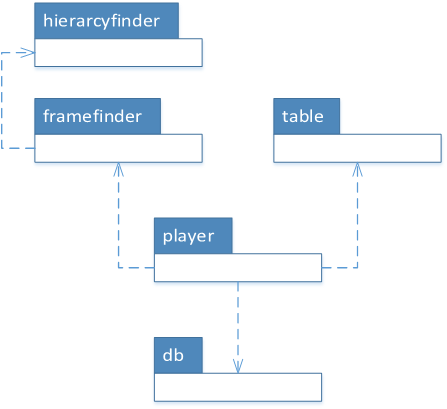
\includegraphics[width=0.4\textwidth]{resources/chapter-4-module-dependecy.png}
	    \caption{Ketergantungan Antar Modul}
		\label{ModuleDependency}
	\end{figure}

	\subsection{Kolaborasi Antar Modul}
	Proses fitur ini akan dilakukan melalui modul \texttt{player} yang dapat menerima perintah pengguna melalui \textit{front-end}. Selanjutnya modul \texttt{framefinder} akan melakukan pendeteksian label dan data secara otomatis pada masing-masing tabel yang terdapat pada \textit{sheet}. Tabel-tabel tersebut didapatkan melalui modul \texttt{hierarchyfinder}. Selanjutnya, pada saat menerima perintah penyimpanan, modul \texttt{table} akan dipanggil oleh \texttt{player}. Jika data masukan sudah benar, maka modul \texttt{mysql} akan melakukan pennyimpanan ke dalam basis data. Kolaborasi antar modul disajikan pada Gambar \ref{ModuleFlow}.

	\begin{figure}[htb]
	    \centering
	    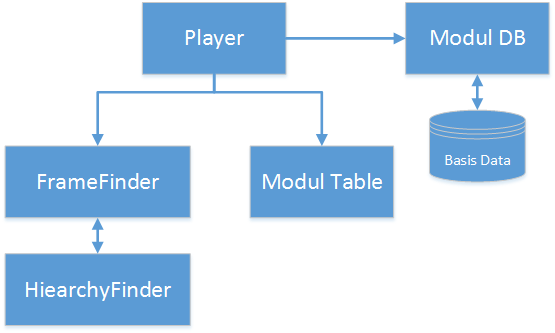
\includegraphics[width=0.5\textwidth]{resources/chapter-4-module-flow.png}
	    \caption{Kolaborasi Antar Modul}
		\label{ModuleFlow}
	\end{figure}

	Pada aplikasi Ethercalc, modul yang ditambahkan akan berada di bawah modul \texttt{player} yang sudah ada. Ilustrasi penempatan modul yang dibuat pada aplikasi EtherCalc yang sudah ada dapat dilihat pada Gambar \ref{ModulePlacing}.

	\begin{figure}[htb]
	    \centering
	    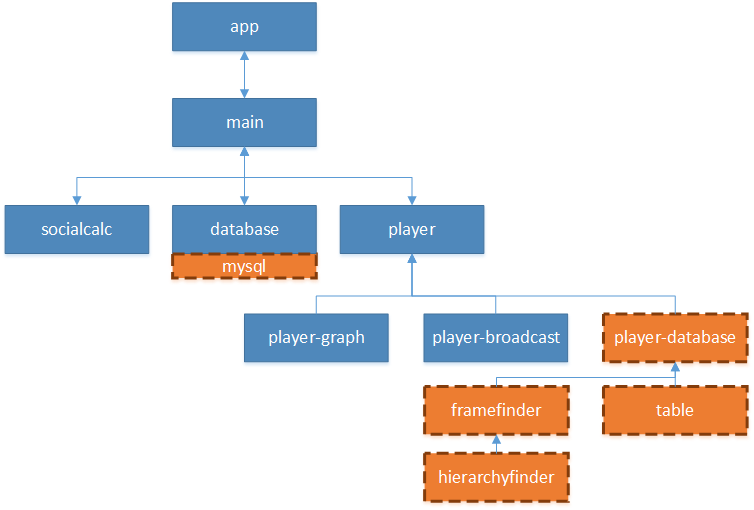
\includegraphics[width=0.6\textwidth]{resources/chapter-4-module-placing.png}
	    \caption{Interaksi dengan Modul yang Sudah Ada}
		\label{ModulePlacing}
	\end{figure}

	\subsection{Arsitektur}
	Aplikasi dibuat dengan menggunakan bantuan Docker sehingga diharapkan dapat dengan mudah dipasang pada berbagai \textit{platform}. Aplikasi terdiri dari tiga \textit{docker container} yakni untuk aplikasi utama, basis data redis, dan basis data MySQL. \textit{File} \texttt{docker-compose.yml} yang dibuat untuk mendefinisikan \textit{docker container} yang digunakan dapat dilihat pada Kode \ref{KodeCompose}

	\begin{lstlisting}[frame=single, basicstyle=\linespread{1}\scriptsize\listingsfont, captionpos=b, caption={Kode pada docker-compose.yml}, label=KodeCompose]
	ethercalc:
	  build: .
	  ports:
	    - "80:8000"
	  links:
	    - redis:redis
	    - mysql:mysql
	  restart: always
	redis:
	  image: redis:latest
	  volumes:
	    - /var/lib/redis:/data
	  command: redis-server --appendonly yes
	  restart: always
	mysql:
	  image: mysql:5.7
	  volumes:
	    - db_data:/var/lib/mysql
	  restart: always
	  environment:
	    MYSQL_ROOT_PASSWORD: root
	    MYSQL_DATABASE: TA
	    MYSQL_USER: user
	    MYSQL_PASSWORD: user
	\end{lstlisting}

	Untuk menyimpan \textit{state} konfigurasi tabel dan \textit{mapping} \textit{metadata table} dengan data pada basis data, digunakan dua tabel basis data yang sudah didefinisikan sebelumnya. Kedua tabel basis data ini dinamakan s\_database\_state dan s\_database\_wlog, kedua tabel ini tidak memiliki keterhubungan. Atribut yang terdapat pada kedua tabel ini dapat dilihat pada diagram struktur basis data pada Gambar \ref{StructureDiagram}.

	\begin{figure}[htb]
	    \centering
	    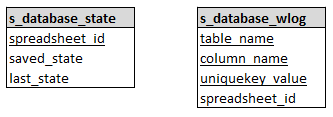
\includegraphics[width=0.5\textwidth]{resources/chapter-4-architect-db.png}
	    \caption{Diagram Struktur Tabel Penyimpanan Konfigurasi}
		\label{StructureDiagram}
	\end{figure}

	\textit{metadata table} yang ditampilkan kepada pengguna akan berasal dari tabel s\_database\_state dan juga disimpan pada tabel tersebut. Kegunaan  s\_database\_wlog adalah mencatat pemetaan data kepada \textit{metadata table} sehingga saat \textit{metadata table} dihapus, data yang berasal dari \textit{metadata table} tersebut dapat juga dihapus.

	Kakas dibuat di atas aplikasi EtherCalc, sehingga akan diimplementasi tambahan modul maupun menggunakan modul yang sudah ada pada EtherCalc. Interaksi antar modul yang dibuat dengan modul yang sudah ada serta dengan data masukan dapat dilihat pada Gambar \ref{ArchDiagram}.

	\begin{figure}[htb]
	    \centering
	    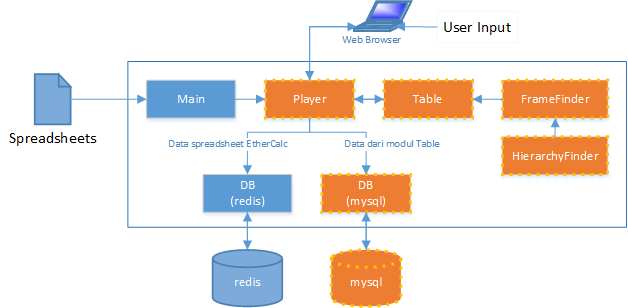
\includegraphics[width=0.7\textwidth]{resources/chapter-4-architecture.png}
	    \caption{Diagram Arsitektur Aplikasi}
		\label{ArchDiagram}
	\end{figure}

	Pada diagram arsitektur terlihat bahwa masih terdapat dua basis data yakni redis dan MySQL. Hal ini dilakukan agar data mengenai format dan cara ditampilkan pada aplikasi EtherCalc tetap disimpan pada basis data redis sedangkan data yang ingin dikumpulkan dan digabungkan oleh pengguna dimasukkan pada basis data relasional MySQL.

	% Modul-modul dan fitur dibuat di atas aplikasi EtherCalc, sehingga arsitektur kakas akan mengikuti arsitektur aplikasi EtherCalc yang telah dijelaskan pada Subbab \ref{TeknologiSpreadsheet}.

\section{Implementasi}
Implementasi dilakukan dengan membangun modul yang telah dijabarkan pada Subbab \ref{KebutuhanModul} dengan menggunakan bahasa Javascript, menyesuaikan dengan modul lain yang telah ada pada aplikasi EtherCalc. Pada bagian ini akan dijelaskan antarmuka dan modul-modul yang diimplementasikan.
	\subsection{Antarmuka}
	Antarmuka aplikasi pada Tugas Akhir ini mengikuti antarmuka yang telah ada sebelumnya pada aplikasi EtherCalc. Fitur baru yang ditambahkan akan menempati menu baru pada bagian atas antarmuka dengan nama `Data Collector`. Antarmuka awal dapat dilihat pada Gambar \ref{Antarmuka1}.

	\begin{figure}[htb]
	    \centering
	    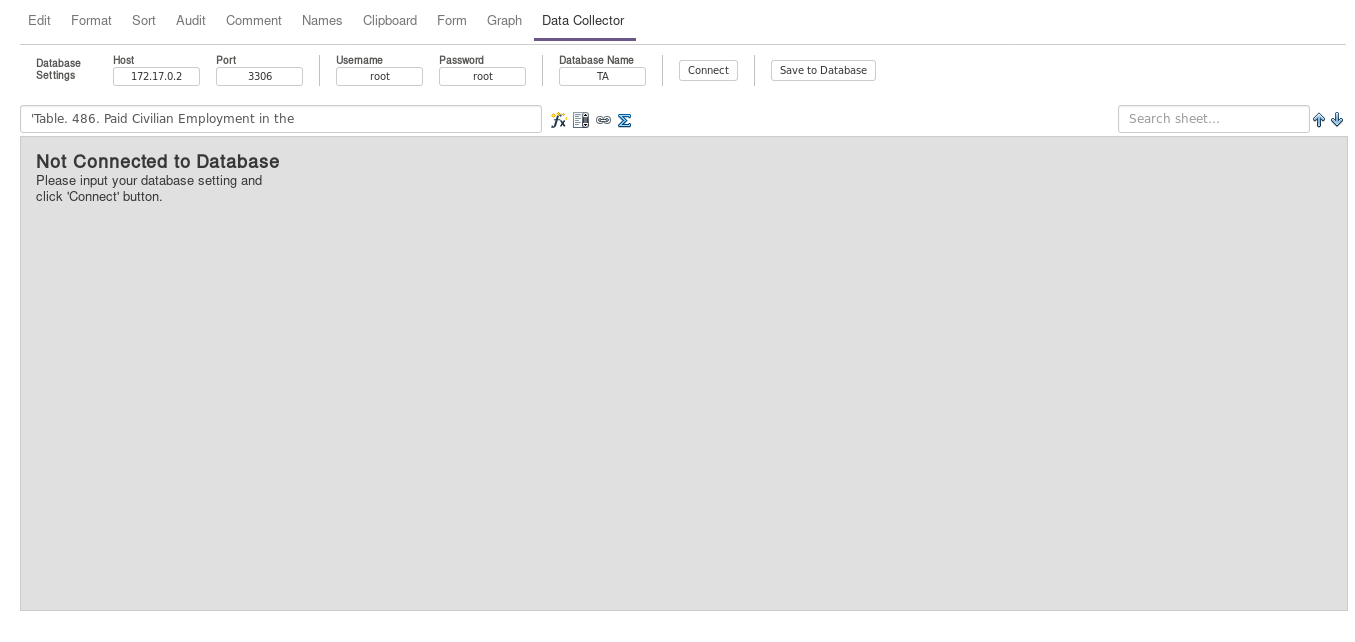
\includegraphics[width=1.0\textwidth]{resources/chapter-4-interface-1.png}
	    \caption{Antarmuka Awal}
		\label{Antarmuka1}
	\end{figure}

	Terdapat dua bagian utama pada antarmuka ini, yang pertama adalah area pengaturan basis data dimana pengguna bisa dapat mengatur koneksi ke basis data yang diinginkan. Yang kedua adalah area tempat \textit{metadata table} dapat ditambahkan dan dikurangi berdasarkan masukan pengguna. Pada bagian kiri area \textit{metadata table}, terdapat dua pilihan metode untuk membuat \textit{metadata table} yakni secara manual maupun otomatis. Kedua area ini dapat dilihat pada Gambar \ref{Antarmuka2}.

	\begin{figure}[htbp]
	    \centering
	    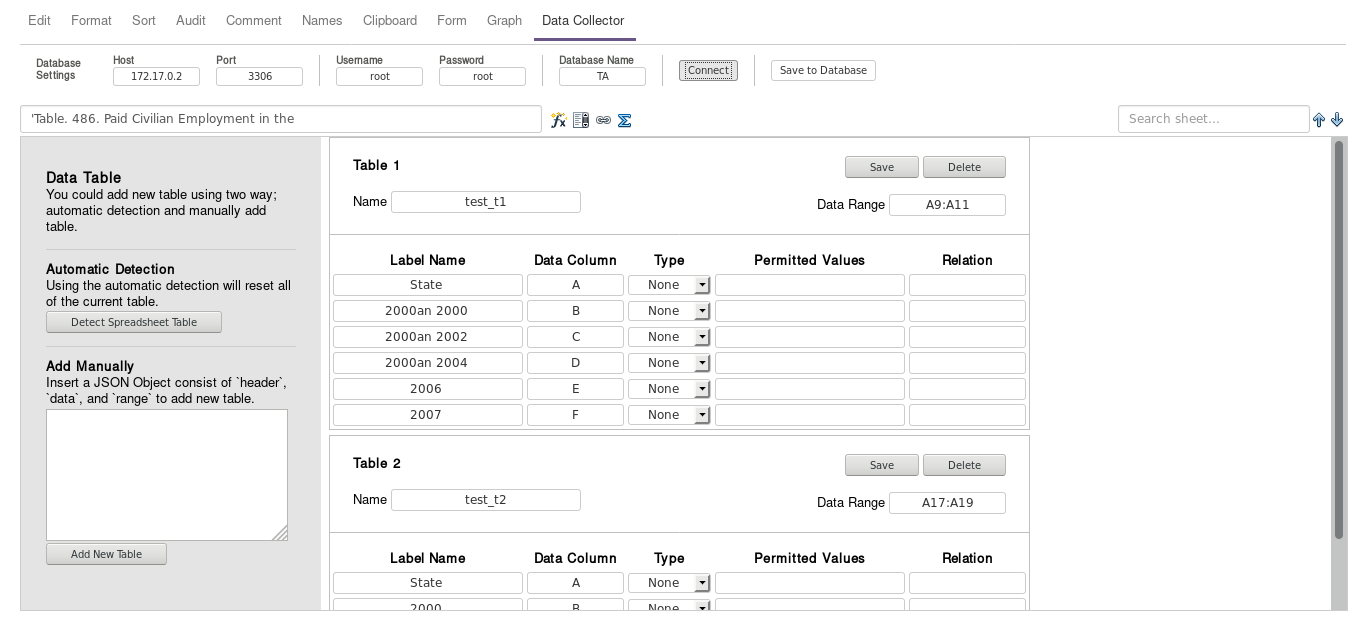
\includegraphics[width=1.0\textwidth]{resources/chapter-4-interface-2.png}
	    \caption{Antarmuka \textit{metadata table}}
		\label{Antarmuka2}
	\end{figure}

	Pada bagian \textit{metadata table}, pengguna dapat menentukan nama label, tipe data, nilai-nilai yang diizinkan, dan relasinya terhadap kumpulan sel lain untuk suatu kolom data. Pengguna dapat juga mengubah nama tabel tujuan ke basis data serta menghapus \textit{metadata table}. Jika terjadi kesalahan pada saat validasi, pengguna akan diberikan pesan kesalahan dan diharapkan untuk memperbaiki data pada sel yang dianggap memiliki kesalahan. Interaksi ini dapat dilihat pada Gambar \ref{Antarmuka3}.

	\begin{figure}[htbp]
	    \centering
	    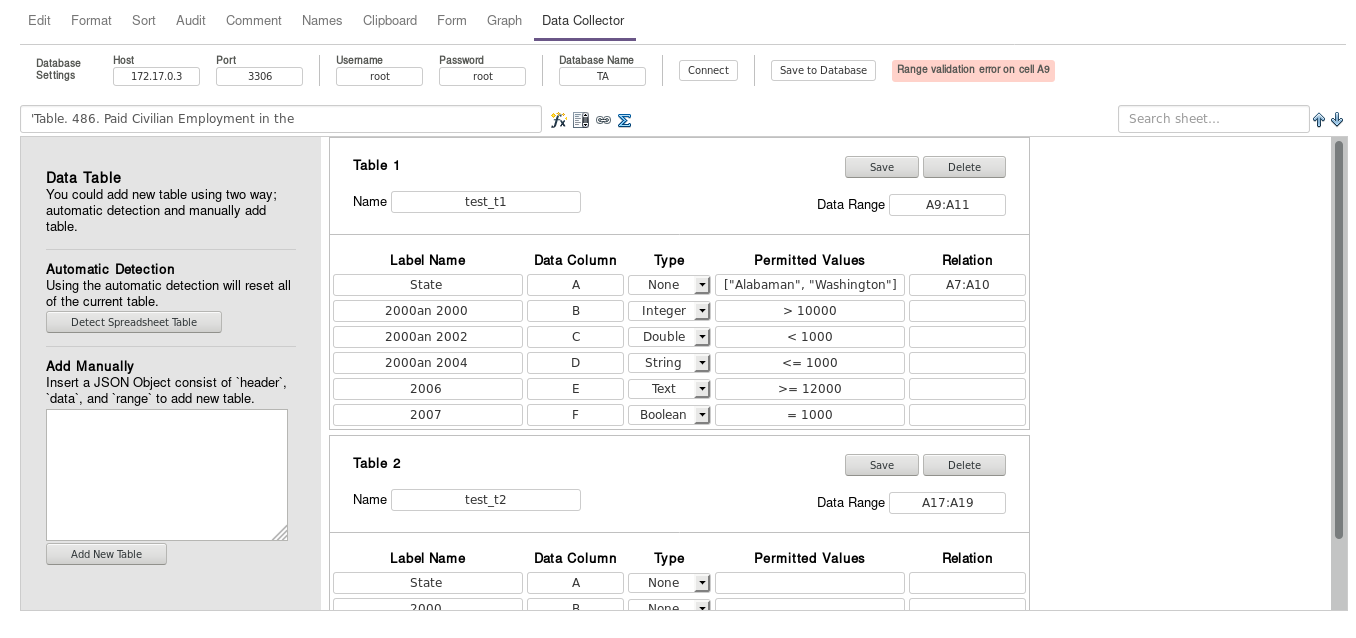
\includegraphics[width=1.0\textwidth]{resources/chapter-4-interface-3a.png}
	    \caption{Antarmuka Perubahan \textit{metadata table}}
		\label{Antarmuka3}
	\end{figure}
	
	\subsection{Modul Main}
	Modul \texttt{Main} merupakan modul yang sudah ada pada aplikasi EtherCalc. Untuk mengimplementasi kakas, modul ini dikembangkan lagi dengan menambahkan beberapa \textit{endpoint} API yang dibutuhkan. Seluruh API ini akan dipanggil melalui modul \texttt{Player}. API yang ditambahkan pada Tugas Akhir ini adalah:
	\begin{enumerate}
		\item \texttt{POST /\_database/connect} \\
		Digunakan untuk melakukan pengecekan koneksi ke basis data. Parameter yang dibutuhkan adalah:
		\begin{itemize} 
			\item host: \textit{host} basis data.
			\item port: \textit{port} basis data.
			\item user: \textit{user} basis dat yang digunakan.
			\item password: \textit{password} untuk \textit{user} yang digunakan.
			\item database: nama \textit{database} yang digunakan.
		\end{itemize}
	
		\item \texttt{POST /\_database/state} \\
		Digunakan untuk melakukan penyimpanan \textit{state} \textit{metadata table}. Parameter yang dibutuhkan adalah:
		\begin{itemize} 
			\item tables: data \textit{metadata table} dalam bentuk JSON.
			\item setting: pengaturan koneksi ke basis data yang dipilih berupa JSON Object.
		\end{itemize}

		\item \texttt{POST /\_database/state/[spreadsheet\_id]} \\
		Digunakan untuk mendapatkan data \textit{state} \textit{metadata table} pada suatu \textit{spreadsheet}. Parameter yang dibutuhkan adalah::
		\begin{itemize}
			\item setting: pengaturan koneksi ke basis data yang dipilih berupa JSON Object.
		\end{itemize}

		\item \texttt{POST /\_database/create} \\
		Digunakan untuk melakukan penyimpanan data yang telah dikumpulkan sesuai dengan aturan pada \textit{metadata table}. Parameter yang dibutuhkan adalah:
		\begin{itemize} 
			\item table: data dari \textit{metadata table} yang telah diubah menjadi bentuk relasional dalam bentuk JSON.
			\item setting: pengaturan koneksi ke basis data yang dipilih berupa JSON Object.
		\end{itemize}
	
		\item \texttt{GET /\_framefinder/[spreadsheet\_id]/[start\_col]/[end\_col]\\/[start\_row]/[end\_row]} \\
		Digunakan untuk mendapatkan hasil pencarian label dan data diantara kolom dan baris tertentu.

		\item \texttt{GET /\_hierarchical/[spreadsheet\_id]} \\
		Digunakan untuk mendapatkan perkiraan kelompok sel yang merupakan suatu kesatuan tabel.	
	\end{enumerate}

	\subsection{Modul Player}
	Modul \texttt{player} merupakan modul yang menjembatani masukan pengguna dari yang berasal dari \textit{front-end} sehingga dapat diterima oleh modul yang berada di \textit{back-end}. Modul ini hanya terdiri dari satu kelas utama yakni kelas \texttt{player} yang berisi fungsi-fungsi yang dapat dipanggil oleh \textit{front-end} yang dapat dilihat pada Lampiran A.
	
	\subsection{Modul DB}
	Modul basis data digunakan sebagai antarmuka modul lain untuk melakukan operasi I/O basis data. Pada Tugas Akhir ini, basis data yang digunakan adalah MySQL. Modul ini hanya terdiri dari satu kelas utama yakni kelas \texttt{mysql}. Kelas ini memiliki tugas sebagai penghubung kakas ke basis data MySQL yang dipilih. Fungsi-fungsi yang terdapat pada kelas ini dapat dilihat pada Lampiran A.

	Tabel akan dibuat pada basis data yang ditentukan, setiap tabel merepresentasikan suatu tabel pada \textit{spreadsheet} yang ditentukan oleh pengguna. \textit{Header} yang didefinisikan oleh pengguna pada \textit{spreadsheet} akan dijadikan \textit{column} pada tabel basis data, tipe yang dibentuk mengikuti masukan pengguna. Tiap baris data yang ada dibawah \textit{header} pada \textit{spreadsheet} akan ditranslasikan menjadi bentuk relasional agar dapat dimasukan ke dalam tabel.
	
	\subsection{Modul Hierarchyfinder}
	Modul \texttt{hierarchyfinder} menggunakan algoritma kNN jenis \textit{hierarchical clustering} untuk dapat mengetahui mana yang merupakan suatu kesatuan tabel pada suatu \textit{sheet}. Modul ini dapat menentukan tabel-tabel yang terdapat pada suatu \textit{sheet} yang selanjutnya akan dilakukan identifikasi label oleh modul \texttt{framefinder}. Algoritma \textit{hierarchical clustering} yang digunakan menganggap setiap sel pada \textit{spreadsheet} merupakan suatu node. Sel-sel yang bersebelahan dengan sel tersebut akan dianggap tetangga sehingga memiliki jarak sama dengan 0. Sel yang digabungkan dengan sel lain akan dihitung sebagai satu \textit{node}. Aturan perhitungan jarak antar \textit{node} dapat dilihat pada kode di Kode \ref{KodeJarak}.\\

	\begin{lstlisting}[frame=single, basicstyle=\linespread{1}\scriptsize\listingsfont, captionpos=b, caption={Perhitungan Jarak \textit{Node}}, label=KodeJarak]
	# Fungsi cellDistance(v1, v2)
	# Parameter pada fungsi adalah v1 (node 1) dan v2 (node 2)
	t = new Table null, null
	colD = t.GetCellCol(v1[0]) - t.GetCellCol(v2[0])
	rowD = t.GetCellRow(v1[0]) - t.GetCellRow(v2[0])

	# Jika sel saling bertetangga tetapi bukan secara diagonal
	# Jika bertetangga, jarak kedua sel adalah 0
	if colD == 0
		if rowD == 1 or rowD == -1
			return 0
	if rowD == 0
		if colD == 1 or colD == -1
			return 0

	# Jika tidak, cek apakah sel bertetangga secara diagonal
	# Jika bertetangga, jarak kedua sel adalah 0
	leftTop = [[v1[1], v1[2]], [v2[1], v2[2]]]
	leftBot = [[v1[1], (v1[2] + v1[4])], [v2[1], (v2[2] + v2[4])]]
	righTop = [[(v1[1] + v1[3]), v1[2]], [(v2[1] + v2[3]), v2[2]]]
	righBot = [[(v1[1] + v1[3]), (v1[2] + v1[4])], [(v2[1] + v2[3]), (v2[2] + v2[4])]]

	if (leftTop[0][0] == righTop[1][0] and leftTop[0][1] == righTop[1][1])
		return 0
	if (leftBot[0][0] == righBot[1][0] and leftBot[0][1] == righBot[1][1])
		return 0

	if (leftTop[1][0] == righTop[0][0] and leftTop[1][1] == righTop[0][1])
		return 0
	if (leftBot[1][0] == righBot[0][0] and leftBot[1][1] == righBot[0][1])
		return 0

	if (leftTop[0][0] == leftBot[1][0] and leftTop[0][1] == leftBot[1][1])
		return 0
	if (righTop[0][0] == righBot[1][0] and righTop[0][1] == righBot[1][1])
		return 0

	if (leftTop[1][0] == leftBot[0][0] and leftTop[1][1] == leftBot[0][1])
		return 0
	if (righTop[1][0] == righBot[0][0] and righTop[1][1] == righBot[0][1])
		return 0

	# Jika tidak juga, hitung jarak menggunakan teknik Euclidian
	dist = Math.sqrt(Math.pow((v2[1] + (v2[3]/2)) - (v1[1] + (v1[3]/2)), 2) + Math.pow((v2[2] + (v2[4]/2)) - (v1[2] + (v1[4]/2)), 2));
	return dist
	\end{lstlisting}

	Hasil dari pengelompokan ini berupa kelompok-kelompok tabel pada \textit{spreadsheet}. Setiap tabel yang teridentifikasi selanjutnya akan dicari bagian \textit{header} dan \textit{label} menggunakan modul \texttt{framefinder}.

	\subsection{Modul Framefinder}
	Modul \texttt{framefinder} melakukan pengidentifikasian terhadap tabel yang ada sehingga dapat diketahui baris yang merupakan \textit{header} dan \textit{data}. Implementasi modul ini dilakukan dengan mengikuti implementasi yang dilakukan pada penelitian yang dilakukan oleh Chen \citep{Chen2013}. Modul ini terdiri dari 5 kelas yang dapat dilihat pada Lampiran A.

	\begin{enumerate}
		\item Kelas LoadSheet\\
		Kelas ini melakukan pengambilan data pada \textit{spreadsheet} dengan cara membaca file \textit{spreadsheet} dan membentuk representasi kelas yang dibutuhkan. Kelas ini memiliki satu atribut utama yakni cmysheet yang merupakan kelas MySheet. Fungsi-fungsi yang terdapat pada kelas ini dapat dilihat pada Lampiran A.

		\item Kelas MySheet\\
		Kelas MySheet merupakan kelas yang merepresentasikan \textit{sheet} pada \textit{spreadsheet} yang dipilih. Kelas ini memiliki 4 atribut yang dapat dilihat pada Lampiran A. Pada kelas ini terdapat 3 fungsi yang dapat dilihat juga pada Lampiran A.

		\item Kelas MyCell\\
		Kelas MyCell merupakan kelas yang merepresentasikan sel pada suatu \textit{sheet}. Kelas ini memiliki 17 atribut yang dapat dilihat pada Lampiran A.
	\end{enumerate}

	% Pada kelas ini terdapat 3 fungsi yang dapat dilihat pada Tabel \ref{FungsiMyCell}.

	% \begin{small}
	% \begin{longtable}{ | p{4cm} | p{9cm} | }
	%     \caption{Fungsi pada Kelas MyCell}
	%     \label{FungsiMyCell}\\ \hline
	%     \centering\bfseries{Nama Fungsi} & \centering\bfseries{Deskripsi} \tabularnewline \hline
	%     \endfirsthead
	%     \hline
	%     \centering\bfseries{Nama Fungsi} & \centering\bfseries{Deskripsi} \tabularnewline \hline
	%     \endhead
	%     writestrAlignstyle & Mendapatkan representasi \textit{string} untuk \textit{align} pada sel. Digunakan pada saat penulisan ke dalam file untuk dibaca pada algoritma CRF.\\ \hline
	%     writestrBorderstyle & Mendapatkan representasi \textit{string} untuk \textit{border} pada sel. Digunakan pada saat penulisan ke dalam file untuk dibaca pada algoritma CRF.\\ \hline
	%     getIndents & Digunakan untuk menentukan nilai atribut indentasi dengan menghitung seberapa dalam indentasi pada konten.\\ \hline
	% \end{longtable}
	% \end{small}

	\subsubsection{Kelas FeatureSheetRow}
	Kelas ini bertugas untuk melakukan ekstraksi fitur pada tiap baris sel yang telah dikumpulkan dari \textit{spreadsheet}. Fitur-fitur yang diambil untuk setiap barisnya dapat dilihat pada Lampiran A.

	Fitur-fitur di atas mengikuti fitur yang didefinisikan pada penelitian yang dilakukan oleh Chen \citep{Chen2013}. Fitur-fitur ini akan digunakan dalam perhitungan algoritma CRF.

	\subsubsection{Kelas PredictSheetRows}
	Kelas PredictSheetRows memiliki tugas untuk melakukan konversi fitur-fitur yang telah didapatkan pada kelas FeatureSheetRow menjadi bentuk file teks yang dapat dibaca oleh program CRFPP yang akan menjalankan algoritma CRF pada file tersebut. Contoh file yang dihasilkan oleh kelas ini dapat dilihat pada Kode \ref{KodeFile}.\\

	\begin{lstlisting}[frame=single, basicstyle=\linespread{1}\scriptsize\listingsfont, captionpos=b, caption={File Berisikan Fitur Tiap Baris}, label=KodeFile]
	DeadlineTA.xls____Sheet1____1 1 0 1 0 0 1 0 1 0 0 0 0 0 0 1 0 1 1 0 0 0 0 0 Header
	DeadlineTA.xls____Sheet1____2 0 1 1 0 0 1 0 0 0 0 0 1 0 0 1 0 1 1 0 0 0 0 0 Data
	DeadlineTA.xls____Sheet1____3 0 1 1 0 0 1 0 0 0 0 0 1 0 0 1 0 0 0 0 0 0 0 0 Data
	DeadlineTA.xls____Sheet1____4 0 1 1 0 0 1 0 0 0 0 0 1 0 0 1 0 0 0 0 0 0 0 0 Data
	DeadlineTA.xls____Sheet1____5 0 1 1 0 0 1 0 0 0 0 0 1 0 0 1 0 0 1 0 0 0 0 0 Data
	\end{lstlisting}

	File tersebut ditulis dalam format \texttt{namafile\_namasheet\_bariske [fitur-fitur pada baris] label}. File ini yang akan diolah oleh algoritma dan digunakan untuk memprediksi label dari setiap baris tersebut. Algoritma yang digunakan adalah Conditional Random Field dan menggunakan aplikasi CRFPP yang berjalan eksternal diluar kelas ini untuk membaca file, membaca model, serta memprediski label.

	\subsection{Modul Table}
	Modul \texttt{table} memiliki tugas untuk mengelola tampilan dan isi \textit{metadata table}, melakukan validasi data masukan, dan membuat representasi relasional yang dapat diterima oleh basis data. Modul \texttt{table} hanya memiliki satu kelas yakni kelas \texttt{table}. Kelas ini memiliki 8 atribut yang dapat dilihat pada Lampiran A.	Pada kelas ini terdapat 6 fungsi yang dapat dilihat pada Lampiran A.

	Modul ini berinteraksi langsung dengan modul \texttt{player} pada saat akan melakukan penyimpanan \textit{state} \textit{metadata table} dan menampilkan \textit{metadata table} pada \textit{front-end}. Selain itu, modul ini juga berhubungan dengan modul \texttt{mysql} pada saat melakukan penyimpanan.

\section{Pengujian}
Pengujian dilakukan hanya kepada fitur yang di buat pada Tugas Akhir ini dan tidak kepada aplikasi EtherCalc secara keseluruhan. Pada subbab ini akan dibahas kasus-kasus yang diuji dan hasil dari pengujian tersebut.

	\subsection{Tujuan Pengujian}
	Pada fitur yang dibangun pada Tugas Akhir ini, pengujian yang dilakukan mempunyai tujuan yaitu fitur yang diimplementasi dapat berjalan dengan baik. Pengujian yang dilakukan akan dikaitkan pada kebutuhan-kebutuhan kakas yang telah didefinisikan sebelumnya. Dari pengujian akan dilihat kesesuaian hasil sesungguhnya dengan hasil yang diinginkan.

	% \begin{enumerate}
	% 	\item Fitur yang diimplementasi dapat berjalan dengan baik. Pengujian yang dilakukan akan dikaitkan pada kasus-kasus penggunaan yang dapat terjadi. Dari pengujian akan dilihat kesesuaian hasil sesungguhnya dengan hasil yang diinginkan.
	% 	\item Mencatat waktu eksekusi yang dibutuhkan untuk fitur-fitur yang ditambahkan.
	% \end{enumerate}

	\subsection{Lingkungan Pengujian}
	Pengujian dilakukan pada komputer dengan spesifikasi pada Tabel \ref{LingPengujian}.

	\begin{small}
	\begin{longtable}{ | p{3cm} | p{9cm} | }
	    \caption{Spesifikasi Lingkungan Pengujian}
	    \label{LingPengujian}\\ \hline
	    \centering\bfseries{Komponen} & \centering\bfseries{Deskripsi} \tabularnewline \hline
	    \endfirsthead
	    \hline
	    \centering\bfseries{Komponen} & \centering\bfseries{Deskripsi} \tabularnewline \hline
	    \endhead
		Prosesor & AMD A8-4500M APU with Radeon(tm) HD Graphics 1.90GHz\\ \hline
		Memori Fisik & 12 GB\\ \hline
		\textit{Storage} & 50 GB\\ \hline
		Sistem Operasi & Arch Linux 64-bit\\ \hline
		Docker version & 1.13.1\\ \hline
		\textit{Web browser} & Mozilla Firefox 51.0.1\\ \hline
	\end{longtable}
	\end{small}

	\subsection{Eksekusi Pengujian} \label{skenarioujian}
	Kasus pengujian disesuaikan dengan kebutuhan fungsional dan non-fungsional yang sudah dijelaskan pada Subbab \ref{PerancanganPL}. Setiap kasus uji diberi kode TC-XX dengan XX adalah nomor kasus uji. Daftar kasus uji dapat dilihat pada Tabel \ref{KasusUjiFA}.

	\begin{small}
	\begin{longtable}{ | p{2cm} | p{8cm} | p{3cm} | }
	    \caption{Kasus Uji Fitur Kakas}
	    \label{KasusUjiFA}\\ \hline
	    \centering\bfseries{ID} & \centering\bfseries{Tujuan} & \centering\bfseries{ID kebutuhan terkait} \tabularnewline \hline
	    \endfirsthead
	    \hline
	    \centering\bfseries{ID} & \centering\bfseries{Tujuan} & \centering\bfseries{ID kebutuhan terkait} \tabularnewline \hline
	    \endhead
		TC-01 & Terkoneksi ke basis data MySQL yang dipilih pengguna dan dapat menggunakan basis data tersebut& FR-01, FR-02 \\ \hline
		TC-02 & Mendeteksi label dan data secara otomatis pada \textit{spreadsheet} & FR-04, FR-05 \\ \hline
		TC-03 & Menambahkan \textit{metadata table} secara manual sesuai dengan masukan pengguna & FR-04 \\ \hline
		TC-04 & Pengguna dapat mengubah atribut yang ada pada \textit{metadata table} & FR-06 \\ \hline
		TC-05 & Data dapat dimasukkan ke basis data sesuai dengan \textit{metadata table} & FR-03, FR-09, NF-01 \\ \hline
		TC-06 & Data yang dimasukkan ke basis data berhasil divalidasi sesuai aturan pengguna & FR-07, FR-08, FR-09, NF-01 \\ \hline	
		% TC-07 & Pencatatan \textit{response time} pada fitur yang ditambahkan & FN-03 \\ \hline
	\end{longtable}
	\end{small}

	\subsection{Hasil Pengujian}
	Hasil pengujian dikaitkan dengan ID skenario pengujian yang berkaitan langsung dengan kasus uji yang telah didefinisikan pada Bab \ref{skenarioujian}. Tiap hasil pengujian mempunyai ID skenario terkait, ekspektasi, hasil uji yang dilakukan, dan diterima atau tidaknya hasil pengujian. Hasil pengujian merupakan hasil pelaksanaan skenario yang sudah dibuat dan dapat dilihat pada Lampiran B.